\documentclass[tikz]{article}

\usepackage{tikz}

\usepackage[EULERGREEK]{sansmath}

\newcommand\blurp[{1}]{\foreach \x in {#1}{\x\\}}

\begin{document}


\blurp[{een, twee, drie}]

% \foreach \x in {bla, bli, bloe}{
%   \x \\
% }

\foreach \x in {bla, bli,bloe,1} {
\x \\
}

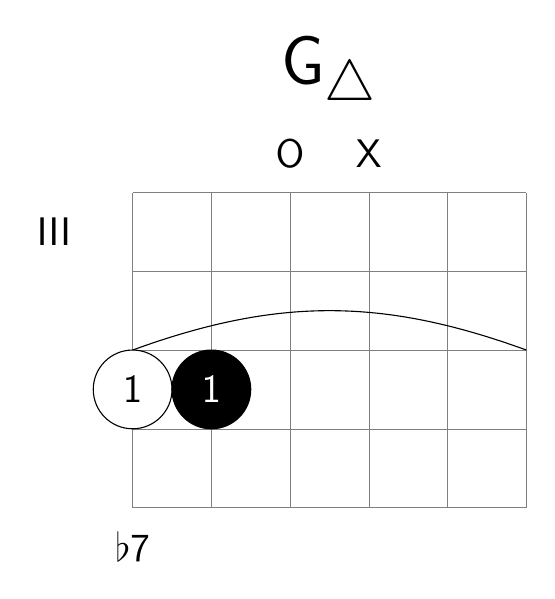
\begin{tikzpicture}[font=\sffamily\sansmath]
\draw[help lines] (0,0) grid (5,4);
\filldraw [fill=white] (0,1.5) circle [radius=0.5];
\draw (0,1.5) node {\Large 1};
\filldraw [fill=black] (1,1.5) circle [radius=0.5];
\draw [color=white] (1,1.5) node {\Large 1};
\draw (-1,3.5) node {\Large III};
\draw (0,2) to[out=20, in=160] (5,2);
\draw (3,4.5) node {\Large X};
\draw (2,4.5) node {\Large O};
\draw (0,-0.5) node {\Large $\flat$7};
\draw (2.5,5.5) node {\Huge G\textsubscript{$\triangle$}};
%\draw[step=0.5, gray, very thin] (-1.4,-1.4) grid (1.4,1.4);
%\draw (0,0) parabola (1,1.5) parabola[bend at end] (2,0);
%\draw (0,0) sin (1,1) cos (2,0) sin (3,-1) cos (4,0) sin (5,1);
\end{tikzpicture}
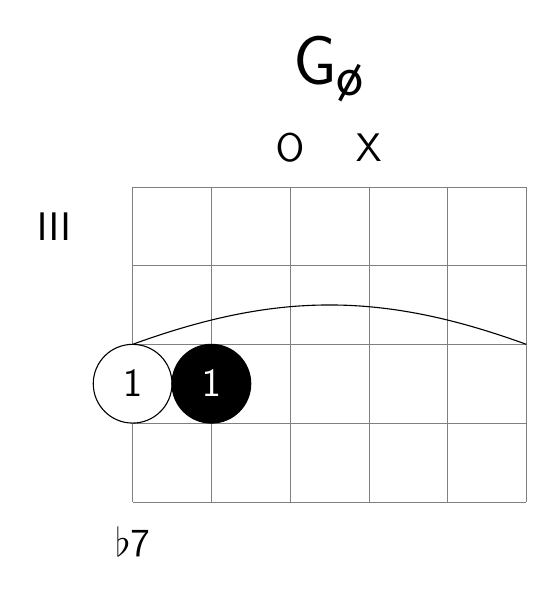
\begin{tikzpicture}[font=\sffamily\sansmath]
\draw[help lines] (0,0) grid (5,4);
\filldraw [fill=white] (0,1.5) circle [radius=0.5];
\draw (0,1.5) node {\Large 1};
\filldraw [fill=black] (1,1.5) circle [radius=0.5];
\draw [color=white] (1,1.5) node {\Large 1};
\draw (-1,3.5) node {\Large III};
\draw (0,2) to[out=20, in=160] (5,2);
\draw (3,4.5) node {\Large X};
\draw (2,4.5) node {\Large O};
\draw (0,-0.5) node {\Large $\flat$7};
\draw (2.5,5.5) node {\Huge G\textsubscript{\o}};
%\draw[step=0.5, gray, very thin] (-1.4,-1.4) grid (1.4,1.4);
%\draw (0,0) parabola (1,1.5) parabola[bend at end] (2,0);
%\draw (0,0) sin (1,1) cos (2,0) sin (3,-1) cos (4,0) sin (5,1);
\end{tikzpicture}
\end{document}
